% Local evidence-integration working draft: 20260930; original 20260914 source retained
% Frozen experiment protocol/artifact revision: 20260815-v1.0.0
\newcommand{\DoNotLoadEpstopdf}{} % All figures are native PDF or PNG.
\documentclass[journal]{IEEEtran}

\usepackage{amsmath,amssymb}
\usepackage{graphicx}
\usepackage{booktabs}
\usepackage{multirow}
\usepackage{cite}
\usepackage{url}
\usepackage{xcolor}
\usepackage{array}
\usepackage{placeins}

\newcommand{\Rone}{R@1}
\newcommand{\Rfive}{R@5}
\newcommand{\Rten}{R@10}
\newcommand{\maptrap}{mAP$_{\mathrm{trap}}$}
\newcommand{\vect}[1]{\boldsymbol{#1}}
\hyphenation{geo-localization cross-view multi-modal}
\raggedbottom
\makeatletter
\setlength{\@dblfptop}{0pt}
\setlength{\@dblfpsep}{10pt}
\setlength{\@dblfpbot}{0pt plus 1fil}
\makeatother
\definecolor{EvidenceBlue}{HTML}{0072B2}
\definecolor{EvidenceTeal}{HTML}{009E73}
\definecolor{EvidenceOrange}{HTML}{D55E00}
\definecolor{EvidenceGray}{HTML}{5C6770}

\title{Independent Content and Style Evidence for UAV--Satellite Retrieval}
\author{Chen~Che}
% Author to supply verified affiliation, corresponding email, and funding before submission.

\begin{document}
\bstctlcite{IEEEAuthorDisplayControl}
\maketitle
\markboth{Local working draft --- 30 September 2026}{Independent Content and Style Evidence}
\begin{center}\footnotesize\itshape
Local working draft: completed-result integration; remaining experiments and final review are pending.
\end{center}

\begin{abstract}
Fixed semantic vocabularies offer a compact way to compare content and
acquisition-style information in UAV--satellite retrieval. We study an
interface with independent per-image encoding: a frozen vision--language model scores
each image against both vocabularies and separate probability encoders fuse
the resulting vectors with a learned visual descriptor. A common
multi-positive training protocol evaluates six input configurations on
University-1652 and SUES-200. Across the 11 official retrieval tasks, the
Full configuration has lower three-seed mean Recall@1 and official
trapezoidal mAP than Visual on 10 tasks; the Street2S exception has low
absolute accuracy. In bidirectional cross-dataset transfer, Full has lower
mean Recall@1 in all 11 target tasks. Seed-1 corruption measurements and
clean-query margin diagnostics characterize these results under explicit
metric and membership definitions. A separate historical study of four
public visual baselines analyzes ranking and score fusion. The completed
comparisons do not support a general accuracy advantage from this frozen
semantic-fusion design and delimit the claims that its conditional
diagnostics can support.
\end{abstract}

\begin{IEEEkeywords}
Cross-view geo-localization, multimodal retrieval, semantic evidence,
unmanned aerial vehicle localization, vision--language models.
\end{IEEEkeywords}

\section{Introduction}
\label{sec:introduction}

Cross-view geo-localization retrieves a geo-referenced image of the place
observed by a query camera \cite{survey2024}. For an unmanned aerial vehicle
(UAV), satellite imagery provides a reference gallery across locations
without a ground-level survey of every route. A UAV image can query this
gallery to identify its scene, and a satellite image can retrieve the
corresponding observations in a UAV image collection. University-1652 and
SUES-200 organize these two directions into identity-based retrieval tasks
\cite{university1652,sues200}. The retrieved scene provides a location
hypothesis for subsequent geometric localization.

Recognizing the same place across views requires more than matching local
appearance. An oblique UAV view exposes building facades and nearby
structures, whereas a satellite view emphasizes roofs, roads, and the
surrounding layout. Flight altitude changes the visible footprint and the
relative scale of these structures. Shadows, vegetation, and sensor response
add further appearance variation. At the same time, different locations may
contain similar buildings, parking areas, or road patterns, as illustrated
in Fig.~\ref{fig:motivation}. A useful descriptor must preserve the scene
information that distinguishes these locations across the view change.

Visual approaches address this problem through descriptor learning and
spatial aggregation. Global encoders summarize the image in a common
embedding space \cite{cvmnet2018,safa2019}. LPN, FSRA, CA-HRS, and SDPL retain
local patterns or align feature regions to represent finer scene structure
\cite{lpn2022,fsra2022,cahrs2023,sdpl2024}. Contrastive training directly
increases the similarity of matching locations while separating other
locations \cite{sample4geo2023}. These methods primarily organize visual
features. Image--text representations provide another source of information:
a score for a concept such as a road intersection or dense building layout
can describe an image through a vocabulary shared by both views.

\begin{figure*}[!t]
  \centering
  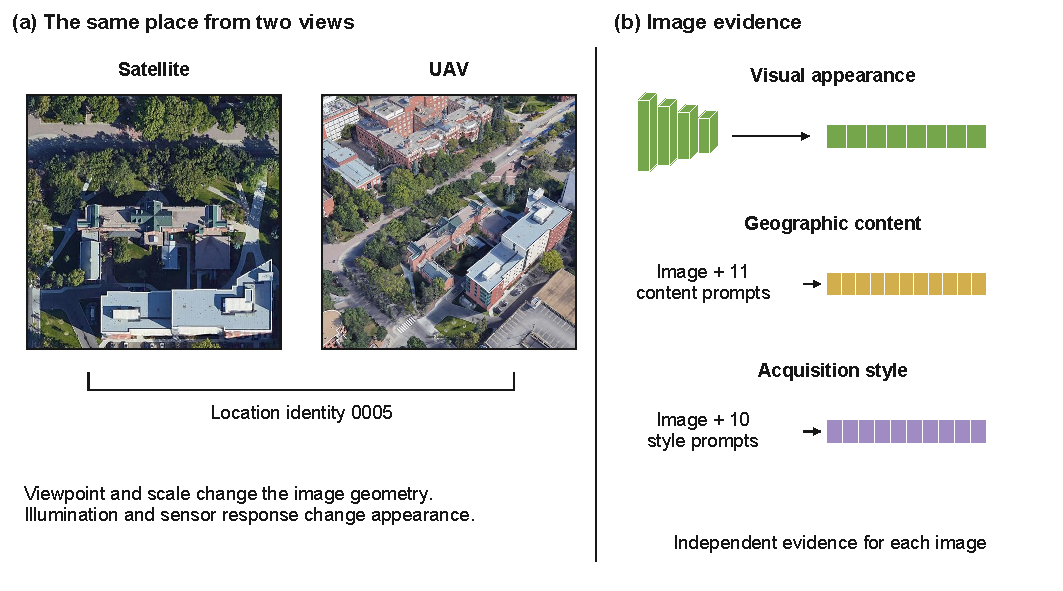
\includegraphics[width=180mm]{figures/journal_20260914/fig01_motivation.pdf}
  \caption{Cross-view observations and image evidence. (a) Satellite and UAV images from location 0005 in University-1652 show changes in geometry and appearance across viewpoints. (b) The visual branch describes image appearance, while frozen CLIP scores each image against 11 content prompts and 10 acquisition-style prompts. The vector glyphs depict the representation structure.}
  \label{fig:motivation}
\end{figure*}

Recent multimodal methods integrate this information at different stages.
CDM-Net uses remote-sensing descriptions in a view-synthesis and
structural-matching pipeline \cite{cdmnet2025}. VLGeo builds attribute-based
descriptions from image triplets and learns cross-view, cross-modal
alignment \cite{vlgeo2026}. These approaches combine semantic input
construction with a dedicated interaction mechanism. We consider a simpler
input interface: a fixed semantic vector computed separately for each
image. This interface allows the reference gallery to be encoded before a
query arrives and exposes the contribution of each semantic input through
branch-level comparisons.

The design distinguishes geographic content from acquisition style.
Content describes visible scene elements, including buildings, roads, and
vegetation. Style describes viewpoint and appearance conditions, including
altitude, illumination, and contrast. Grouping these concepts separately
preserves their different roles when the scores enter the retrieval model.
Content scores can associate visually different observations with common
scene concepts; style scores provide information about the conditions under
which those concepts appear. We use these groups as explicit input
categories and learn their relation to visual features in the fusion head.

Our framework scores each image against two fixed vocabularies using a
frozen vision--language model. A trainable ResNet produces the visual
descriptor, and two independent MLPs encode the content and style scores.
The normalized branch descriptors are concatenated and projected to a common
retrieval space. The query and gallery images share encoder parameters;
each descriptor depends on its own image and the fixed texts. A symmetric
multi-positive contrastive objective accounts for the multiple UAV
observations associated with one location.

Evaluation must also distinguish representation quality from the effect of
the retrieval procedure. Local score normalization can change the leading
match, query expansion can reorder lower-ranked positives, and a smaller
gallery removes difficult competitors. We study these effects with four
public visual baselines and retain the same feature sources within each
comparison. The resulting analysis motivates explicit controls for ranking,
gallery composition, and model combination in semantic-source comparisons.
The contributions of this work are summarized as follows:
\begin{itemize}
  \item We define fixed content and acquisition-style input vectors that are
  constructed separately for each image and can be cached for independent
  query and gallery encoding.
  \item We evaluate six input configurations under one multi-positive
  training protocol, retaining all official tasks and all three seeds.
  The Full-versus-Visual comparison is negative on 10 of 11 official tasks
  for both mean R@1 and mAP, and on all 11 transfer tasks for mean R@1.
  \item We distinguish seed-1 corruption retention from absolute accuracy,
  and shared-query margin strata from variant-specific selective retrieval.
  These diagnostics define the comparison being made without assigning a
  causal explanation or a calibrated-probability interpretation.
  \item We retain a separate analysis of four public visual baselines on
  University-1652, covering ranking rules, gallery size and retrospective
  score fusion under their own trained feature sources.
\end{itemize}

Section~\ref{sec:related} reviews related approaches.
Sections~\ref{sec:method} and \ref{sec:protocol} describe the architecture and
experimental protocol. Section~\ref{sec:semantic-results} reports the
semantic-model results, followed by the separate historical public-baseline
analysis in Section~\ref{sec:public}.

\section{Related Work}
\label{sec:related}

\subsection{Visual Representations for Cross-View Retrieval}

Cross-view retrieval methods preserve scene information through different
feature organizations. CVM-Net learns a common embedding for ground and
aerial imagery \cite{cvmnet2018}. Spatial aggregation and Transformer-based
encoders incorporate structure and context into the descriptor
\cite{safa2019,transgeo2022}. For UAV--satellite retrieval, LPN pools
concentric local regions, FSRA aligns segmented feature regions, CA-HRS
selects hierarchical representations, and SDPL aggregates shifted dense
partitions \cite{lpn2022,fsra2022,cahrs2023,sdpl2024}. Their different spatial
units address the displacement, scale, and appearance changes between
views.

CAMP combines contrastive attribute mining with position-aware partitioning
\cite{camp2024}. DAC combines a domain space alignment module for
fine-grained features with cross-batch scene consistency \cite{dac2024}.

Training objectives provide complementary constraints. Sample4Geo combines
symmetric contrastive learning with negative sampling
\cite{sample4geo2023}. Classifier interaction, causal representation
learning, multilevel alignment, and query-driven feature learning further
shape the cross-view embedding \cite{mccg2024,ccr2024,mean2025,qdfl2025}.
DSTG uses multiscale logit-standardization distillation to transfer a Swin
Transformer teacher to a smaller student \cite{dstg2025}. Its
ground-to-satellite experiments on CVUSA and CVACT address model efficiency
in a different view setting. Our visual branch uses a ResNet with global
pooling, which provides a common visual input for the content and style
branch comparisons.

Recent preprints extend this line of work toward efficiency, geometry, and
cross-dataset transfer. MobileGeo studies hierarchical knowledge
distillation for compact retrieval encoders \cite{mobilegeo2026}.
MGS2-Net incorporates a depth prior into geometric representation learning
\cite{mgs2026v2}, while InfoGeo studies information-theoretic, object-centric
learning for transfer across geo-localization datasets \cite{infogeo2026}.
Their encoder inputs and evaluation settings are retained in the reference
comparisons below.

\subsection{Semantic Inputs and Multimodal Matching}

CLIP learns a common space for image and text embeddings \cite{clip2021}.
In geo-localization, textual information can describe a query, condition an
image-generation stage, or guide feature alignment. GeoText-1652 provides
natural-language descriptions and spatial-relation matching
\cite{geotext2024}. CDM-Net combines perspective transformation,
remote-sensing descriptions, and conditional diffusion before matching
point--line structure in the synthesized view \cite{cdmnet2025}. The
descriptions therefore contribute to both the synthesized image and its
structural representation.

VLGeo generates attribute prompts from triplet images and learns
bidirectional-guided semantic alignment with contrastive supervision
\cite{vlgeo2026}. Its ablations examine modal combinations, description
attributes, language models, and alignment components. We instead use the
image--text encoder to score fixed concepts separately for each image.
Content and style probabilities enter two learned branches alongside the
visual descriptor. The common vocabulary gives every image the same
semantic coordinates and supports independent gallery encoding. This
compact representation captures concept scores; detailed descriptions and
explicit spatial relations provide a richer, different input interface.

\subsection{Environmental Variation and Localization Settings}

Environmental changes affect both image features and semantic scores.
MuSe-Net models environmental style in aerial retrieval
\cite{musenet2024}. EAGLe combines a dual-objective discriminator with a
style-mixture module: adversarial training promotes view and environment
invariance, while feature-statistic mixing broadens the styles encountered
during training \cite{eagle2025}. Our style branch follows a conditioning
approach. It retains the image's acquisition-style scores as auxiliary input
to descriptor fusion. Clean and corrupted-query comparisons measure how
that conditioning changes retrieval under appearance shifts.

Other geo-localization settings produce different outputs or consume
additional observations. Vector-map retrieval uses map geometry,
region-to-point localization links regional and point-level matches, and
iterative rendering combines multiple UAV observations
\cite{vectormap2025,r2ploc2025,rendering2025}. Game4Loc evaluates
continuous-region and non-centered localization \cite{game4loc2025}. The
present study uses ranked whole-image identity retrieval on
University-1652 and SUES-200. We specify gallery composition, query view,
and ranking rules for each comparison because these settings determine the
candidate matches available to a descriptor.

\section{Independent Semantic Evidence Fusion}
\label{sec:method}

\subsection{Task Formulation and Framework Overview}

Let $\mathcal{X}^{q}=\{(x_i^{q},y_i)\}$ and
$\mathcal{X}^{g}=\{(x_j^{g},y_j)\}$ denote query and gallery images, where
$y$ identifies a location. The query and gallery roles are assigned by the
evaluation task; they do not change the image encoder. For active branches
$\mathcal{A}\subseteq\{v,c,s\}$, the descriptor is
\begin{equation}
  \vect{z}=F_\theta(x,\vect{p}^{c}(x),\vect{p}^{s}(x);\mathcal{A})
  \in\mathbb{R}^{d},
  \label{eq:strict-gate}
\end{equation}
where only inputs selected by $\mathcal{A}$ are consumed. Superscripts $v$,
$c$, and $s$ denote visual, content, and style branches. The same parameters
$\theta$ encode the two views independently. We use the stable normalization
\begin{equation}
  \mathcal{N}(\vect{u})=
  \frac{\vect{u}}{\max(\|\vect{u}\|_2,\varepsilon)},
  \qquad \varepsilon=10^{-12}.
  \label{eq:stable-normalization}
\end{equation}
The output is $L_2$-normalized and retrieval sorts cosine scores:
\begin{equation}
  s_{ij}=\vect{z}_i^{q\top}\vect{z}_j^{g},\qquad
  \pi_i=\operatorname{argsort}_{j}^{\downarrow}s_{ij}.
  \label{eq:retrieval-ranking}
\end{equation}
Here $\pi_i$ lists gallery indices in descending similarity order.

Figure~\ref{fig:mechanism} separates offline evidence construction from
trainable retrieval. Frozen CLIP encoders create two probability vectors for
each image. A ResNet branch encodes visual appearance, while two independent
multilayer perceptrons (MLPs) encode content and style probabilities. A
multimodal variant concatenates its normalized branch descriptors and learns
a fusion projection; a single-branch variant returns that branch directly.
Location labels determine positive matches in the training objective, but
are not encoder inputs. At inference, each image is encoded once before
query--gallery similarities are computed.

\begin{figure*}[!t]
  \centering
  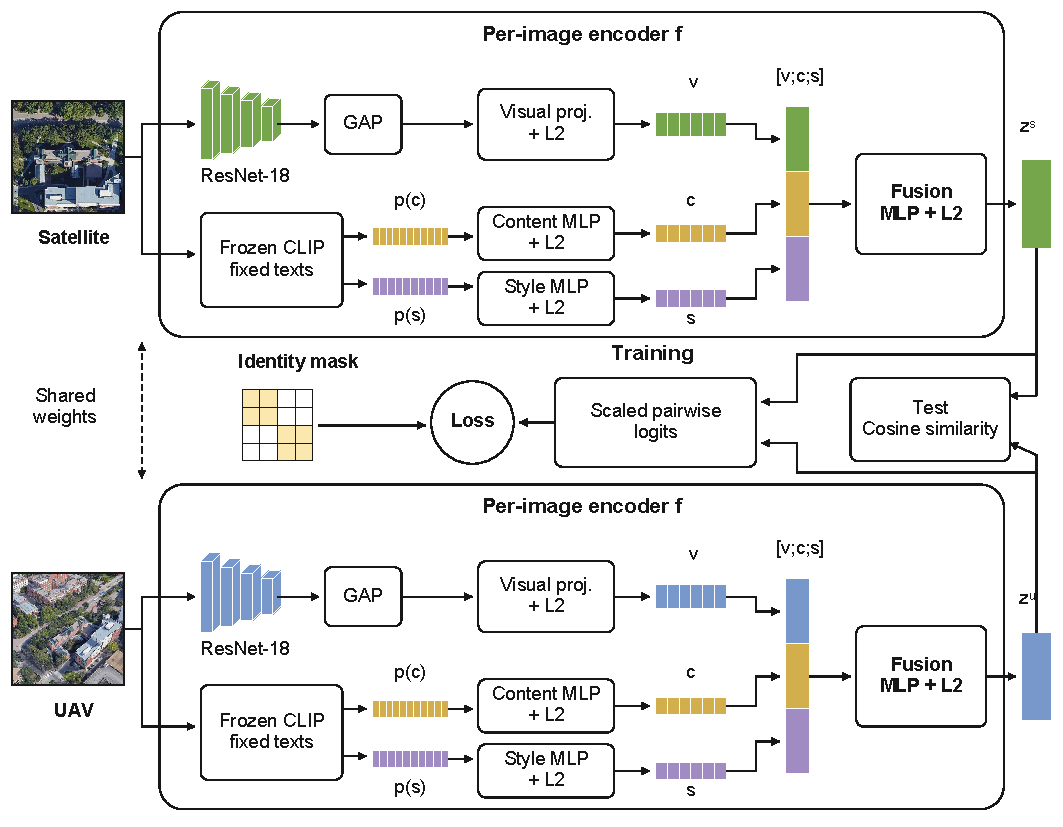
\includegraphics[width=180mm]{figures/journal_20260914/fig02_framework.pdf}
  \caption{Overview of the full visual--content--style retrieval model. Satellite and UAV images follow two independent calls to the same per-image encoder $f$, with shared trainable parameters. ResNet-18 followed by global average pooling and a visual projection produces $\vect{v}$. Frozen CLIP computes separate softmax probability vectors over the fixed content and style vocabularies, which separate MLPs project to $\vect{c}$ and $\vect{s}$. Each branch is $L_2$-normalized. The concatenation $[\vect{v};\vect{c};\vect{s}]$ is projected and normalized to a 512-dimensional descriptor. During training, the two descriptor batches form scaled pairwise logits and a same-identity mask defines the symmetric multi-positive objective. At test time, cosine similarity ranks independently encoded gallery descriptors. Green and blue denote satellite and UAV visual features, amber denotes content, and lavender denotes style.}
  \label{fig:mechanism}
\end{figure*}

\subsection{Fixed Content and Style Evidence}
\label{sec:evidence}

We separate what an image contains from how it is acquired so that their
retrieval effects can be tested separately. The content vocabulary
$\mathcal{C}=\{c_k\}_{k=1}^{11}$ covers campus layout, buildings, roads,
intersections, parking, vegetation, sports fields, open areas, water, dense
layout, and stable spatial layout. The style vocabulary
$\mathcal{S}=\{s_l\}_{l=1}^{10}$ covers UAV/satellite viewpoint, altitude,
shadows, illumination, contrast, sensor gap, and seasonal vegetation.
The two groups define the prompt categories used by the probability
branches. Their scores can be correlated across images.

Frozen OpenAI CLIP ViT-B/32 image and text encoders run in FP16
\cite{clip2021}. For image embedding $\vect{e}(x)$ and text embedding
$\vect{t}(w)$, normalization gives
\begin{equation}
  \hat{\vect{e}}(x)=\frac{\vect{e}(x)}{\|\vect{e}(x)\|_2},\qquad
  \hat{\vect{t}}(w)=\frac{\vect{t}(w)}{\|\vect{t}(w)\|_2}.
  \label{eq:clip-normalization}
\end{equation}
Each vocabulary is scored separately:
\begin{align}
  p_k^{c}(x)
    &=\frac{\exp(\tau\hat{\vect{e}}(x)^\top\hat{\vect{t}}(c_k))}
    {\sum_{r=1}^{11}\exp(\tau\hat{\vect{e}}(x)^\top\hat{\vect{t}}(c_r))},
    \label{eq:content-probability}\\
  p_l^{s}(x)
    &=\frac{\exp(\tau\hat{\vect{e}}(x)^\top\hat{\vect{t}}(s_l))}
    {\sum_{r=1}^{10}\exp(\tau\hat{\vect{e}}(x)^\top\hat{\vect{t}}(s_r))}.
    \label{eq:style-probability}
\end{align}
The frozen scale is $\tau=100$, and the text order is fixed. These are
relative scores normalized within each vocabulary. The vocabulary and its
ordering therefore remain fixed throughout a comparison.

The cache stores $\vect{p}^{c}\in\mathbb{R}^{11}$ and
$\vect{p}^{s}\in\mathbb{R}^{10}$ under each relative image path. CLIP
receives the image pixels and the fixed texts. Training labels are joined
by path when constructing positive pairs for the retrieval objective.
Content-only and style-only variants use the corresponding probability
vector; visual-plus-one-branch variants combine that vector with learned
visual features.

\begin{figure*}[!t]
  \centering
  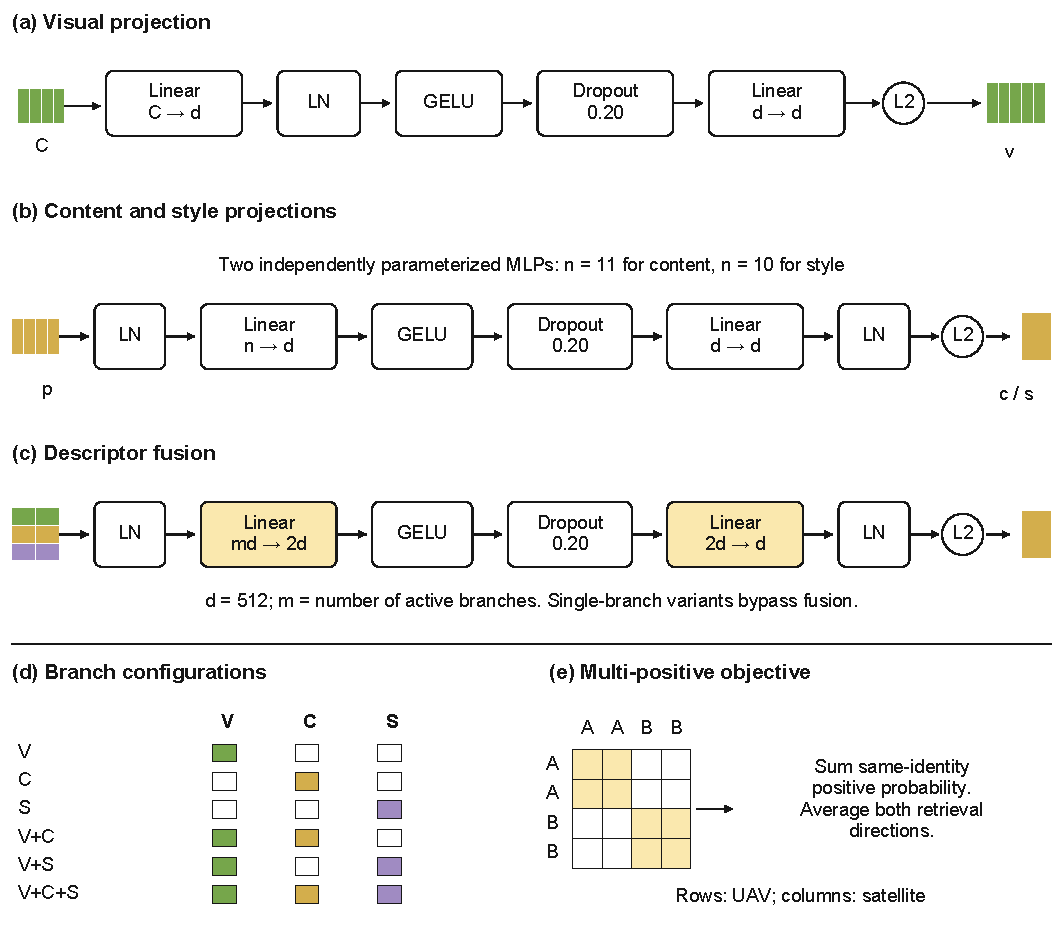
\includegraphics[width=180mm]{figures/journal_20260914/fig03_mechanism.pdf}
  \caption{Projection layers, branch configurations, and the training objective. (a) The visual projection takes $C$-dimensional pooled features, where $C=512$ for ResNet-18 and $C=2048$ for the ResNet-50 sensitivity model. (b) Content and style use distinct MLP parameters with input dimensions $n=11$ and $n=10$, respectively. (c) For $m$ active branches, the fusion head maps $md$ to $2d$ and then $d$, with $d=512$ in the main configuration; a single active branch bypasses this head. LN denotes layer normalization, and $L_2$ denotes normalization of the output vector. (d) The six input configurations. (e) An illustrative four-pair identity mask, in which every same-identity pair contributes to the positive probability mass. The objective averages both retrieval directions.}
  \label{fig:leakage}
\end{figure*}

\subsection{Visual and Probability Encoders}

The visual branch retains a learned image representation beyond the fixed
semantic scores. An ImageNet-initialized ResNet-18 or ResNet-50
\cite{resnet2016} produces a globally pooled feature
$\vect{g}=f_{\mathrm{cnn}}(x)\in\mathbb{R}^{C}$, where $C=512$ or
$C=2048$, respectively. The final classifier is removed, and the globally pooled final feature
map supplies the visual projection. Let $A^a_r(\vect{u})=W^a_r\vect{u}+\vect{b}^a_r$
be an affine layer, $\mathrm{LN}_n$ layer normalization over $n$ entries,
$\sigma$ the Gaussian error linear unit (GELU), and $D_\rho$ dropout with
probability $\rho$. The visual projection is
\begin{align}
  \vect{h}^{v}&=D_\rho\!\left[
    \sigma\!\left(\mathrm{LN}_{d}(A_1^v(\vect{g}))\right)\right],\\
  \vect{z}^{v}&=\mathcal{N}(A_2^v(\vect{h}^{v})).
  \label{eq:visual-projection}
\end{align}
The affine widths are $C\rightarrow d\rightarrow d$. Dropout is active
during training and disabled during evaluation.

The probability branches adapt the low-dimensional fixed scores to the
retrieval space without updating CLIP. For $a\in\{c,s\}$, let $n_c=11$ and
$n_s=10$. Each branch has its own parameters and follows
\begin{align}
  \vect{h}^{a}&=D_\rho\!\left[
    \sigma\!\left(A_1^a(\mathrm{LN}_{n_a}(\vect{p}^{a}))\right)\right],\\
  \vect{z}^{a}&=\mathcal{N}\!\left[
    \mathrm{LN}_{d}(A_2^a(\vect{h}^{a}))\right].
  \label{eq:probability-encoder}
\end{align}
The widths are $n_a\rightarrow d\rightarrow d$. Unlike the visual
projection, a probability MLP normalizes its input before its first affine
layer and applies another layer normalization after its second affine layer.
Figure~\ref{fig:leakage} summarizes the normalized branch descriptors, their controlled fusion, and the positive-mask construction. Each probability branch processes one image, and the fusion head learns
how its scores interact with the visual descriptor.

\subsection{Branch Configuration and Descriptor Fusion}

Keeping separate encoders makes the source comparisons explicit, but their
outputs must still be combined for joint retrieval. Table~\ref{tab:variants}
defines the active branch set for each variant. The branch configuration is
fixed before training. For a multimodal
variant with $m=|\mathcal{A}|$, the concatenation follows the order visual,
content, style with inactive branches omitted:
\begin{equation}
  \vect{h}_{\mathcal{A}}=
  \vect{z}^{a_1}\Vert\cdots\Vert\vect{z}^{a_m}\in\mathbb{R}^{md}.
  \label{eq:active-concatenation}
\end{equation}
The fusion head is
\begin{align}
  \vect{r}&=D_\rho\!\left[
    \sigma\!\left(A_1^f(\mathrm{LN}_{md}(\vect{h}_{\mathcal{A}}))\right)\right],\\
  \vect{z}&=\mathcal{N}\!\left[\mathrm{LN}_{d}(A_2^f(\vect{r}))\right],
  \label{eq:fusion-head}
\end{align}
with widths $md\rightarrow2d\rightarrow d$. For $m=1$, the fusion head is
absent and $\vect{z}=\vect{z}^{a_1}$. Thus every variant has the same output
dimension, while multimodal variants learn how their active sources interact.

\begin{table}[t]
\centering
\caption{Input configurations. All active encoders are learned under the
same retrieval objective; the CLIP evidence remains frozen.}
\label{tab:variants}
\small
\begin{tabular}{lccc}
\toprule
Variant & Visual & Content & Style\\
\midrule
visual          & \checkmark &            &            \\
content         &            & \checkmark &            \\
style           &            &            & \checkmark \\
visual+content  & \checkmark & \checkmark &            \\
visual+style    & \checkmark &            & \checkmark \\
full            & \checkmark & \checkmark & \checkmark \\
\bottomrule
\end{tabular}
\end{table}

The primary contrasts are visual+content versus visual, visual+style versus
visual, and full versus each two-branch variant. These comparisons test the effect of adding evidence under a common
training protocol. The output width is shared, while the added probability
encoders and fusion layers increase the parameter count.

\subsection{Multi-Positive Contrastive Training}

Several UAV observations can correspond to one location, so treating only
the diagonal pair as positive would penalize valid same-location matches.
Following the contrastive retrieval formulation \cite{sample4geo2023}, we
therefore optimize the probability mass assigned to all positives. A batch
contains $B_I=16$ identities and $B_K=4$ query instances per identity, giving
$B=B_I B_K$. Each query receives a same-identity satellite image selected
deterministically from its path, epoch, and seed. For trainable log-scale
$\alpha$, the logits and positive mask are
\begin{align}
  L_{ij}&=\gamma\vect{z}^{q\top}_i\vect{z}^{g}_j,\qquad
  M_{ij}=\mathbb{1}[y_i=y_j],\\
  \gamma&=\exp[\operatorname{clamp}(\alpha,\log 5,\log 100)].
  \label{eq:logits-mask}
\end{align}
The scale is initialized with $\alpha=\log(1/0.07)$ and lies in $[5,100]$
during the forward pass. The directional objective is
\begin{equation}
  \mathcal{L}_{q\rightarrow g}=
  \frac{1}{B}\sum_i\left[
  \log\sum_j e^{L_{ij}}-\log\sum_{j:M_{ij}=1}e^{L_{ij}}\right].
  \label{eq:multi-positive}
\end{equation}
Both sums are evaluated with log-sum-exp; the batch is rejected if an anchor
has no positive. The training objective is
\begin{equation}
  \mathcal{L}=\tfrac12
  (\mathcal{L}_{q\rightarrow g}+\mathcal{L}_{g\rightarrow q}),
  \label{eq:symmetric-loss}
\end{equation}
where the reverse direction uses the transposed logits and mask. The same objective is used for every input configuration, holding the
supervision rule fixed across branch comparisons.

\begin{figure*}[!t]
  \centering
  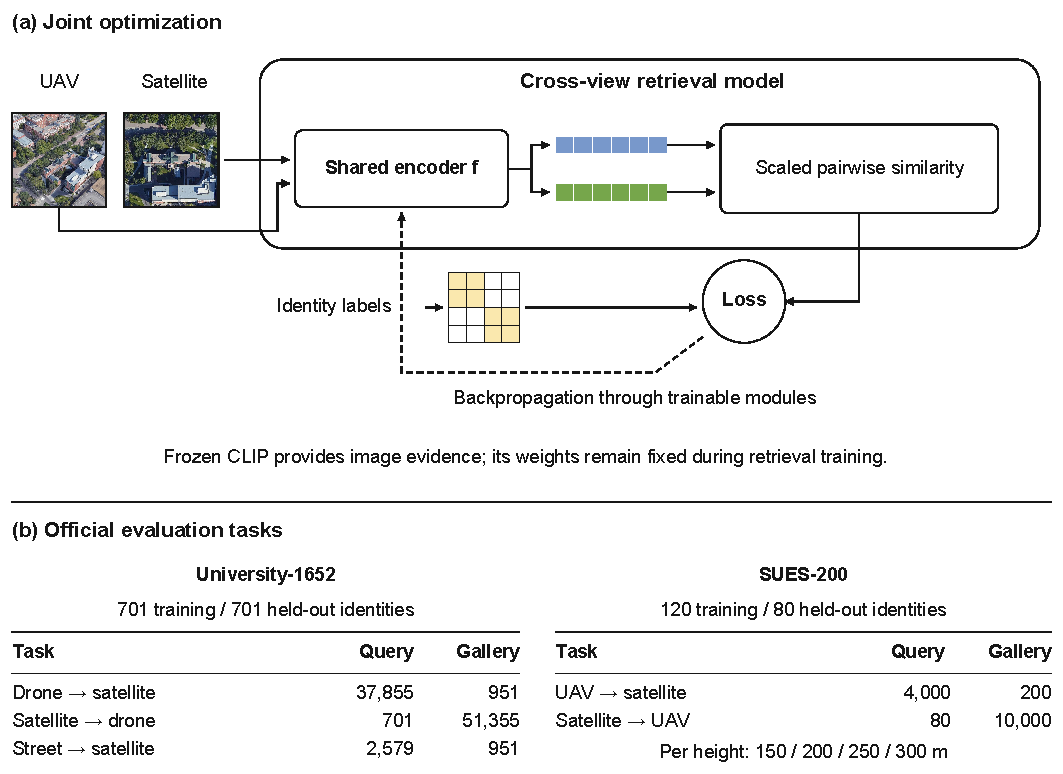
\includegraphics[width=180mm]{figures/journal_20260914/fig04_protocol.pdf}
  \caption{Joint optimization and official retrieval tasks. (a) UAV and satellite images are independently encoded using shared parameters. Scaled descriptor similarities and the same-identity mask define the multi-positive loss; gradients update the visual backbone and projection/fusion modules while CLIP remains frozen. (b) Official query and gallery counts. University-1652 has 701 training identities, 701 held-out identities, and 250 additional distractor identities. SUES-200 uses the fixed 120/80 training/test identity split and evaluates each of four UAV heights separately; each gallery retains all 200 identities.}
  \label{fig:tasks}
\end{figure*}

\section{Evaluation Settings}
\label{sec:protocol}

The protocol compares content and style inputs under the same image
encoder, training schedule, and retrieval tasks. Section~\ref{sec:public}
reports a complementary analysis of four public visual baselines with
fixed feature sources. The completed semantic-model evidence comprises
42 fits and 231 official run--task evaluations, followed by transfer,
seed-1 corruption and clean-query diagnostics. Later external-comparison
and efficiency results are not represented as completed experiments here.
Author-checkpoint re-evaluation and independent training for CAMP and DAC
remain unfinished. Their published results are distinct from the completed
project evaluations.

\subsection{Datasets and Retrieval Tasks}

\textbf{University-1652.} The semantic-model protocol uses the 701 official
training identities, with 40,513 drone/street training queries and 701
same-identity satellite positives. The identity-disjoint test defines
drone-to-satellite (D2S), satellite-to-drone (S2D), and street-to-satellite
(Street2S) retrieval \cite{university1652}. D2S uses 37,855 queries from 701
identities against 951 satellite images; S2D uses 701 queries against 51,355
drone images; Street2S uses 2,579 queries against 951 satellites. Every gallery
retains 701 target identities and 250 distractor identities. The completed
public-baseline experiments concern D2S and S2D only.

\textbf{SUES-200.} The fixed manifest assigns 120 identities to training and
80 to testing \cite{sues200}. A semantic-model fit uses 24,000 UAV images
from four heights and 120 training satellite images. Separate retrieval
tasks are defined at 150, 200, 250, and 300\,m in both directions. At each
height, UAV-to-satellite retrieval has 4,000 held-out UAV queries and 200
satellite candidates; satellite-to-UAV retrieval has 80 held-out satellite
queries and 10,000 UAV candidates. The full galleries retain all 200
identities, including the 120 training identities as distractors. Results
are specified per height and direction rather than combined with a
duplicated overall score. Figure~\ref{fig:tasks} summarizes both datasets.

\subsection{Reference Methods and Published Settings}

Table~\ref{tab:literature_context} summarizes author-reported results with
the corresponding input resources and evaluation setting. MEAN and the
MobileGeo core use RGB retrieval inputs. CDM-Net introduces textual
descriptions and synthesized views, and MGS2-Net uses a depth prior.
MobileGeo's multi-view postprocessing is listed separately from its core
encoder. The two VLGeo rows use the UAV-VLL extension with RGB-only and
RGB-plus-text inputs. Grouping these settings preserves the distinction
between encoder performance and additional resources available to the
retrieval pipeline. The supplementary material reports flight-height
comparisons on SUES-200 and the University-1652-to-SUES-200 transfer setting.

\begin{table*}[t]
\centering
\caption{Author-reported retrieval results (\%) on University-1652 and its UAV-VLL extension, grouped by input and evaluation setting.}
\label{tab:literature_context}
\fontsize{9}{10.5}\selectfont
\setlength{\tabcolsep}{3.3pt}
\renewcommand{\arraystretch}{1.12}
\begin{tabular}{lllrrrr}
\toprule
Method & Input / protocol & Source & \multicolumn{2}{c}{UAV $\rightarrow$ satellite} & \multicolumn{2}{c}{Satellite $\rightarrow$ UAV} \\
\cmidrule(lr){4-5}\cmidrule(lr){6-7} & & & R@1 & AP & R@1 & AP \\
\midrule
MEAN & RGB, 384 & \cite{mean2025} & 93.55 & 94.53 & 96.01 & 92.08 \\
MobileGeo (core) & RGB, 224; distillation & \cite{mobilegeo2026} & 93.87 & 94.83 & 95.72 & 92.57 \\
\midrule
CDM-Net & Text / generated view, 512 & \cite{cdmnet2025} & 95.13 & 96.04 & 96.68 & 94.05 \\
MGS2-Net (v2) & Depth prior, 336 & \cite{mgs2026v2} & 97.60 & 98.03 & 98.86 & 97.25 \\
\midrule
MobileGeo (+MSRM) & Multi-view postprocessing & \cite{mobilegeo2026} & 97.15 & 97.50 & 95.58 & 96.27 \\
\midrule
VLGeo (RGB only) & UAV-VLL RGB, 224 & \cite{vlgeo2026} & 93.15 & 96.03 & 92.01 & 95.25 \\
VLGeo (RGB + text) & UAV-VLL RGB + text, 224 & \cite{vlgeo2026} & 98.57 & 99.17 & 98.14 & 98.98 \\
\bottomrule
\end{tabular}
\par\vspace{2pt}\begin{minipage}{\textwidth}\fontsize{9}{10.5}\selectfont Input size is in pixels. Horizontal groups separate RGB encoders, auxiliary inputs, multi-view postprocessing, and the UAV-VLL extension. Sources: MEAN Table I; CDM-Net Table III; MGS2-Net v2 Table 1; MobileGeo v3 Table I; VLGeo Table II.\end{minipage}
\end{table*}


\subsection{Training and Model Comparisons}

The main configuration uses ResNet-18 \cite{resnet2016}, a 512-dimensional
descriptor, dropout 0.20 \cite{dropout2014}, resizing to 256 pixels and
cropping to 224 pixels. Training is configured for 80 epochs with AdamW
\cite{adamw2019}, base learning rate $3\times10^{-4}$, backbone learning-rate
multiplier 0.1, weight decay $10^{-4}$, gradient clipping at 5, and mixed
precision \cite{mixedprecision2018}. Five warm-up epochs precede cosine
annealing without restarts, using the cosine form in \cite{sgdr2017}.
The predetermined final epoch is evaluated without early stopping or
test-based checkpoint selection. In this no-validation protocol, the
training code names the final completed checkpoint \texttt{best.pt}; the
filename does not denote selection by validation or test performance. Every training query is scheduled at least
once per epoch; the identity sampler and batch construction are specified in
Section~\ref{sec:method}.

The main matrix comprises six input configurations on two datasets with
three seeds, giving 36 completed fits. Six further seed-1 full-model fits vary the backbone
to ResNet-50 or the descriptor width to 256 or 1024 on each dataset. The
single-source models test whether a vocabulary alone carries location
information; the partial and full models test its incremental effect.
QDFL, FSRA, SDPL, CCR, and MCCG remain external visual-comparison targets
\cite{qdfl2025,fsra2022,sdpl2024,ccr2024,mccg2024}; this working draft does
not report those pending comparisons as completed results. The supplementary
material specifies the fit matrix, sampler counts, and reproducibility
records.

\subsection{Metrics and Statistical Analysis}

The protocol specifies Recall@1/5/10/20 and the public University-1652
evaluator's trapezoidal mean average precision, denoted \maptrap.
Mean reciprocal rank (MRR), per-query rank, top-1 margin, parameter count,
peak memory, encoding time, and ranking time provide secondary diagnostics.
The reporting unit for the three-seed comparisons is the task-level mean
and sample standard deviation. The integrated semantic main and transfer
tables are descriptive and do not infer significance from SD. The query
diagnostic audit did not independently resample the retained bootstrap
intervals, which are not used here as new inferential evidence.

For the separate completed public-baseline comparisons, 95\% intervals use 10,000
query-paired bootstrap resamples unless stated otherwise \cite{efron1979}.
Top-1 correctness is compared using two-sided exact McNemar tests
\cite{mcnemar1947,fay2010exact}, with Holm correction \cite{holm1979} within each declared
family: 12 directional method pairs for exact reproduction and 32
method--direction--rule comparisons for ranking sensitivity. Comparisons
require identical query paths and labels. Because D2S contains repeated
queries per location, the selected-fusion analysis also reports
identity-cluster bootstrap sensitivity. That analysis treats location as the resampling unit. The selected subset
and its evaluation queries are held fixed within these resamples. The
supplementary material details the estimands and implementation.

\subsection{Corruption Protocol}

The robustness protocol holds galleries clean and corrupts every official
query image before re-encoding it. Gaussian noise, Gaussian blur, reduced
brightness, and reduced contrast are adaptations of ImageNet-C corruption
families \cite{commoncorruptions2019}. The implemented brightness perturbation
darkens images; these family names do not imply identical transformations or
severity parameters to ImageNet-C. Center occlusion and rotation are
author-defined transformations. Each has five fixed severities. The protocol pairs the visual and full seed-1 models with their
clean-reference evaluations. Full uses cached CLIP evidence for clean
queries and online CLIP evidence for corrupted queries, so its observed
change combines pixel perturbation with a change in evidence path. The
64-image clean diagnostic had no numerical equivalence gate. Results are
seed-1 descriptive comparisons, not multi-seed robustness estimates.

% Completed adopted summaries only; new tables format stored values without scientific recomputation.
\section{Semantic-Model Results}
\label{sec:semantic-results}

The completed fixed-protocol evaluation covers 42 completed training runs
and 231 run--task evaluations: 36 main fits across six input configurations,
two datasets and three seeds, plus six seed-1 sensitivity fits. The main
comparisons retain all 11 official tasks, including Street2S and each SUES-200
height and retrieval direction. Task-level summaries weight seeds 1, 2 and 3
equally and report their sample standard deviation (SD), not a confidence
interval. No overall score pools tasks, directions or heights.

\subsection{Official Retrieval Across Input Configurations}

Tables~\ref{tab:semantic-r1} and \ref{tab:semantic-map} report all six
configurations. Full has lower mean R@1 and official trapezoidal mAP than
Visual on 10 of the 11 tasks. For University-1652 D2S, mean R@1 is
32.300\% for Full and 37.864\% for Visual; for S2D, it is 44.175\% and
54.303\%, respectively. All eight SUES-200 tasks have the same direction
of difference for both metrics. Street2S is the exception: Full reaches
0.969\% R@1 and 2.267\% mAP, compared with 0.788\% and 1.906\% for
Visual. Its low absolute performance remains material to the interpretation.
These descriptive comparisons do not support a general retrieval-accuracy
advantage for the frozen Full configuration.

\begin{table*}[!t]
\centering
\caption{Official R@1 (\%) for all six input configurations. Cells show equally weighted seed-1/2/3 mean $\pm$ sample SD. V+C and V+S denote visual-plus-content and visual-plus-style. SD is descriptive, not a confidence interval. Values are rounded to three decimals; a positive value that would round to zero is shown as $<0.001$. An actual zero remains 0.000.}
\label{tab:semantic-r1}
\footnotesize
\setlength{\tabcolsep}{3pt}
\begin{tabular}{lrrrrrr}
\toprule
Task & Visual & Content & Style & V+C & V+S & Full \\
\midrule
University D2S & $37.864\pm1.011$ & $0.822\pm0.012$ & $0.475\pm0.004$ & $32.549\pm0.245$ & $31.278\pm0.203$ & $32.300\pm0.347$ \\
University S2D & $54.303\pm3.425$ & $1.522\pm0.218$ & $0.095\pm0.082$ & $45.364\pm0.622$ & $44.223\pm2.487$ & $44.175\pm1.539$ \\
University Street2S & $0.788\pm0.234$ & $0.129\pm0.022$ & $0.026\pm0.022$ & $1.112\pm0.281$ & $1.112\pm0.090$ & $0.969\pm0.039$ \\
\midrule
SUES U150$\to$S & $35.558\pm2.766$ & $1.758\pm0.029$ & $0.175\pm0.025$ & $28.017\pm3.838$ & $27.067\pm0.526$ & $28.433\pm1.468$ \\
SUES S$\to$U150 & $57.500\pm3.750$ & $4.583\pm0.722$ & $0.000\pm0.000$ & $44.167\pm5.637$ & $46.667\pm1.909$ & $47.917\pm0.722$ \\
SUES U200$\to$S & $42.975\pm1.664$ & $2.417\pm0.038$ & $0.117\pm0.029$ & $34.083\pm4.280$ & $35.417\pm0.581$ & $33.625\pm1.210$ \\
SUES S$\to$U200 & $63.333\pm2.602$ & $6.250\pm1.250$ & $0.833\pm0.722$ & $50.417\pm4.732$ & $49.167\pm4.018$ & $55.000\pm5.449$ \\
SUES U250$\to$S & $46.958\pm1.363$ & $2.875\pm0.087$ & $0.400\pm0.066$ & $37.642\pm4.525$ & $37.908\pm2.225$ & $36.692\pm1.646$ \\
SUES S$\to$U250 & $69.167\pm3.146$ & $5.833\pm0.722$ & $2.083\pm0.722$ & $52.500\pm4.507$ & $55.833\pm2.602$ & $57.083\pm4.018$ \\
SUES U300$\to$S & $49.708\pm0.326$ & $3.592\pm0.290$ & $0.475\pm0.050$ & $39.967\pm4.194$ & $39.183\pm1.830$ & $38.433\pm0.818$ \\
SUES S$\to$U300 & $73.750\pm3.750$ & $9.583\pm0.722$ & $0.000\pm0.000$ & $58.333\pm2.602$ & $58.750\pm0.000$ & $58.333\pm1.443$ \\
\bottomrule
\end{tabular}
\end{table*}

\begin{table*}[!t]
\centering
\caption{Official trapezoidal mAP (\%) for all six input configurations. Cells show equally weighted seed-1/2/3 mean $\pm$ sample SD. V+C and V+S denote visual-plus-content and visual-plus-style. SD is descriptive, not a confidence interval. Values are rounded to three decimals; a positive value that would round to zero is shown as $<0.001$. An actual zero remains 0.000.}
\label{tab:semantic-map}
\footnotesize
\setlength{\tabcolsep}{3pt}
\begin{tabular}{lrrrrrr}
\toprule
Task & Visual & Content & Style & V+C & V+S & Full \\
\midrule
University D2S & $43.653\pm0.950$ & $1.788\pm0.015$ & $1.155\pm0.009$ & $38.621\pm0.288$ & $37.246\pm0.314$ & $38.448\pm0.269$ \\
University S2D & $35.620\pm1.324$ & $0.740\pm0.005$ & $0.326\pm0.004$ & $29.100\pm0.409$ & $28.551\pm0.606$ & $28.970\pm0.270$ \\
University Street2S & $1.906\pm0.208$ & $0.670\pm0.020$ & $0.432\pm0.030$ & $2.324\pm0.230$ & $2.273\pm0.127$ & $2.267\pm0.110$ \\
\midrule
SUES U150$\to$S & $43.900\pm2.627$ & $5.280\pm0.031$ & $1.696\pm0.046$ & $36.685\pm3.679$ & $35.353\pm0.405$ & $36.634\pm1.210$ \\
SUES S$\to$U150 & $39.523\pm2.134$ & $4.051\pm0.020$ & $1.439\pm0.050$ & $30.765\pm1.844$ & $30.890\pm0.383$ & $33.178\pm1.148$ \\
SUES U200$\to$S & $51.074\pm1.310$ & $6.072\pm0.035$ & $1.670\pm0.076$ & $42.450\pm4.112$ & $42.930\pm0.494$ & $41.635\pm0.787$ \\
SUES S$\to$U200 & $48.755\pm1.197$ & $4.267\pm0.068$ & $1.441\pm0.079$ & $36.588\pm3.132$ & $37.785\pm0.834$ & $38.964\pm1.137$ \\
SUES U250$\to$S & $54.655\pm1.479$ & $6.702\pm0.055$ & $1.980\pm0.091$ & $45.651\pm4.233$ & $45.464\pm1.906$ & $44.590\pm1.590$ \\
SUES S$\to$U250 & $52.298\pm1.569$ & $3.722\pm0.107$ & $1.557\pm0.078$ & $40.865\pm2.895$ & $40.467\pm0.873$ & $42.746\pm1.360$ \\
SUES U300$\to$S & $57.203\pm0.622$ & $7.884\pm0.268$ & $2.129\pm0.040$ & $47.787\pm4.142$ & $46.911\pm1.705$ & $46.412\pm1.279$ \\
SUES S$\to$U300 & $55.070\pm0.369$ & $4.423\pm0.132$ & $1.563\pm0.041$ & $44.238\pm4.189$ & $42.523\pm1.206$ & $44.500\pm0.652$ \\
\bottomrule
\end{tabular}
\end{table*}


The content-only and style-only columns retain the standalone vocabulary
results, while V+C and V+S retain both partial combinations. The complete
matrix permits comparison of the observed input configurations without
selecting favorable tasks or seeds. The additional ResNet-50 and
256/1024-dimensional Full settings are reported with the corresponding
512-dimensional seed-1 reference in the supplementary material. Each
sensitivity setting has one fit per dataset; these are not three-seed
estimates or capacity-matched causal tests of semantic information.

\subsection{Cross-Dataset Transfer}

The transfer evaluation reuses Visual and Full from three source-training
seeds in both dataset directions, giving 12 source-model evaluations and
66 seed--task records. University-1652-trained models are evaluated on the
eight SUES-200 target tasks; SUES-200-trained models are evaluated on the
three University-1652 tasks. Training-dataset direction is distinct from
the target task's query-to-gallery direction.

Table~\ref{tab:semantic-transfer} retains all 22 task--variant groups and
their R@1, official mAP and MRR summaries. Full has lower mean R@1 in all
11 target tasks. Mean mAP and MRR are also lower except for the
SUES-200-to-University-1652 Street2S task, where the saved Full-minus-Visual
differences are 0.040 percentage points for mAP and 0.105 scaled MRR
points. Full Street2S R@1 is 0.233\% with an actual sample SD of zero,
compared with 0.258\% for Visual. The small positive rank-sensitive
differences do not establish a transfer advantage or statistical significance.

\begin{table*}[!t]
\centering
\caption{Cross-dataset transfer: all target tasks, with Visual (V) and Full (F) shown separately. Cells are three-seed mean $\pm$ sample SD. R@1 and official mAP are percentages; MRR$\times100$ is scaled reciprocal rank, not accuracy percent. SD is not a confidence interval. Training-dataset direction is given by the group headings. Values are rounded to three decimals; a positive value that would round to zero is shown as $<0.001$. An actual zero remains 0.000.}
\label{tab:semantic-transfer}
\footnotesize
\setlength{\tabcolsep}{3pt}
\begin{tabular}{lrrrrrr}
\toprule
& \multicolumn{2}{c}{R@1 (\%)} & \multicolumn{2}{c}{mAP (\%)} & \multicolumn{2}{c}{MRR$\times100$} \\
Target task & V & F & V & F & V & F \\
\midrule
\multicolumn{7}{l}{\textit{SUES-200-trained $\to$ University-1652}} \\
University D2S & $11.009\pm0.117$ & $8.178\pm0.609$ & $14.861\pm0.063$ & $11.655\pm0.700$ & $18.714\pm0.038$ & $15.133\pm0.809$ \\
University S2D & $25.678\pm1.753$ & $18.260\pm1.244$ & $9.543\pm0.467$ & $6.967\pm0.438$ & $33.549\pm1.667$ & $25.885\pm2.271$ \\
University Street2S & $0.258\pm0.098$ & $0.233\pm0.000$ & $0.704\pm0.112$ & $0.743\pm0.045$ & $1.149\pm0.142$ & $1.254\pm0.091$ \\
\midrule
\multicolumn{7}{l}{\textit{University-1652-trained $\to$ SUES-200}} \\
SUES U150$\to$S & $19.142\pm2.331$ & $14.592\pm0.927$ & $24.537\pm2.395$ & $19.659\pm0.666$ & $29.932\pm2.497$ & $24.727\pm0.663$ \\
SUES S$\to$U150 & $19.583\pm4.018$ & $12.917\pm1.909$ & $12.802\pm1.671$ & $9.085\pm0.738$ & $25.403\pm3.849$ & $18.488\pm2.094$ \\
SUES U200$\to$S & $23.900\pm2.718$ & $16.067\pm0.797$ & $29.546\pm2.784$ & $21.625\pm0.707$ & $35.193\pm2.883$ & $27.183\pm0.660$ \\
SUES S$\to$U200 & $26.250\pm5.000$ & $15.417\pm1.443$ & $16.867\pm3.354$ & $12.097\pm0.558$ & $33.665\pm5.416$ & $21.401\pm1.810$ \\
SUES U250$\to$S & $27.275\pm2.368$ & $18.608\pm0.986$ & $32.975\pm2.463$ & $24.333\pm0.777$ & $38.675\pm2.575$ & $30.058\pm0.598$ \\
SUES S$\to$U250 & $30.000\pm3.750$ & $20.417\pm2.602$ & $21.294\pm2.895$ & $15.254\pm0.355$ & $36.850\pm3.121$ & $26.658\pm3.145$ \\
SUES U300$\to$S & $29.950\pm2.792$ & $19.533\pm1.102$ & $35.602\pm2.919$ & $25.274\pm0.971$ & $41.255\pm3.059$ & $31.014\pm0.851$ \\
SUES S$\to$U300 & $34.583\pm5.637$ & $19.583\pm1.909$ & $24.482\pm2.544$ & $16.477\pm0.371$ & $40.242\pm5.121$ & $26.014\pm0.605$ \\
\bottomrule
\end{tabular}
\end{table*}


\subsection{Query Corruption and Conditional Diagnostics}

The corruption block evaluates Visual and Full at seed 1 under six
transformation families and five severities on all 11 tasks, with clean
galleries. It contains 660 corrupted task evaluations and 22 clean
task--variant references. The retained-percentage curves use
$100\,m_{\mathrm{corrupt}}/m_{\mathrm{clean}}$ with each variant's own clean
metric. Higher retention therefore does not imply higher absolute corrupted
accuracy. Values above 100\% remain valid observations, and the analysis is
descriptive without multi-seed SD or significance claims. For Full, clean
evaluation uses cached CLIP evidence whereas corrupted queries use online
CLIP evidence; the comparison includes this evidence-path change as well as
pixel perturbation. The 64-image clean diagnostic did not impose a numerical
equivalence gate.

The clean-query diagnostics address a different question: how retrieval
outcomes vary with the margin between the leading two cosine scores. T4
uses the same Visual-defined margin-quartile membership for Visual and
Full in each task and seed. Of its 132 margin strata, the 48 SUES-200
satellite-to-UAV strata contain 20 queries each and are descriptive under
the registered minimum of 100 queries. This is a Visual-anchored conditional
comparison, not a causal explanation of the overall differences.

T5 instead lets each variant select its own margin-ranked subset. Selective
risk is one minus R@1 among the selected queries; coverage-constrained
success divides selected-and-correct queries by the common full query count.
Equal selected counts do not imply equal memberships. The saved all-prefix
AURC is distinct from an area inferred from ten displayed coverage points.
The fixed normalized margin score and its ECE diagnostic do not establish
posterior probabilities or fitted calibration. These conditional diagnostics
do not replace the official and transfer comparisons above. The
supplementary material specifies their denominators and evidence limits.


\section{Historical Visual-Baseline Retrieval Analysis}
\label{sec:public}

This separate historical analysis evaluates four public visual baselines
on University-1652, beginning with full-gallery reproduction and then
examining ranking rules, gallery size and score combination. Its trained
feature sources and retrospective fusion are distinct from the semantic
configurations in Section~\ref{sec:semantic-results}; their gains are not
results of the proposed semantic fusion. Within this block, each comparison
uses the same four trained feature sources.

\begin{figure*}[!t]
  \centering
  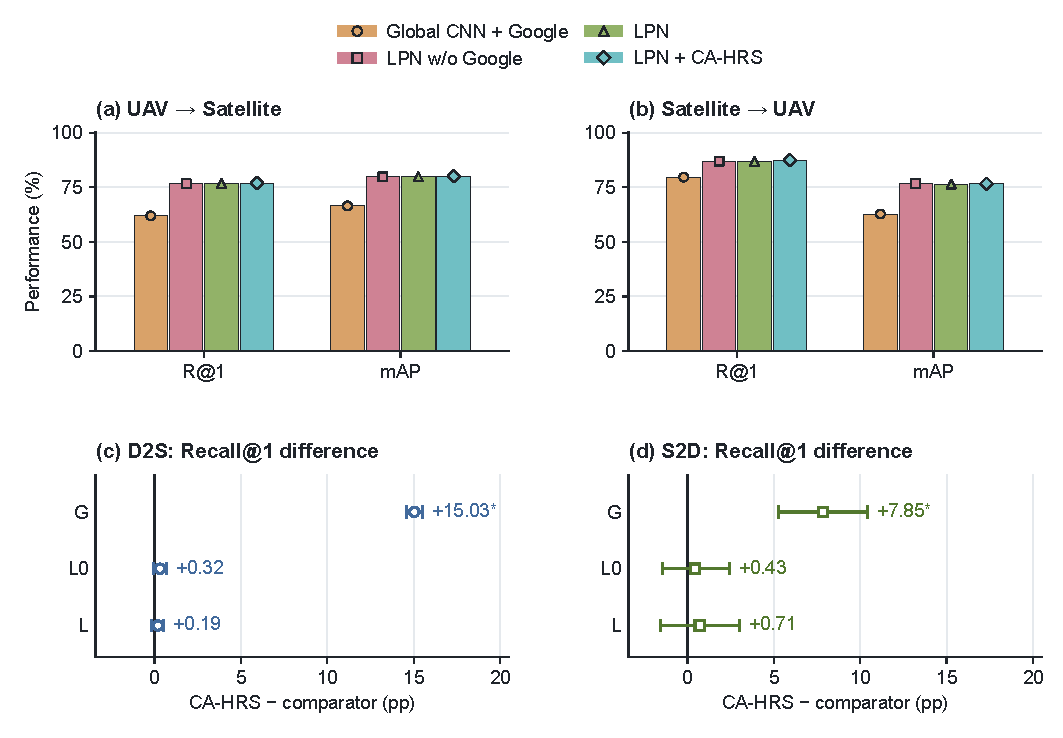
\includegraphics[width=180mm]{figures/journal_20260914/fig05_exact_effects.pdf}
  \caption{Exact full-gallery performance and paired effects on University-1652. Grouped bars compare Recall@1 and official trapezoidal mean average precision (mAP) for four public visual baselines in (a) D2S and (b) S2D, using a common 0--100\% performance scale. (c,d) CA-HRS-minus-comparator Recall@1 differences for D2S and S2D, with query-paired 95\% bootstrap confidence intervals from 10,000 resamples. Asterisks mark exact McNemar comparisons with Holm-adjusted $p<0.05$ in the retained 12-comparison family. G: Global CNN + Google; L0: LPN without Google; L: LPN; C: LPN + CA-HRS. D2S and S2D denote drone-to-satellite and satellite-to-drone retrieval.}
  \label{fig:exact-public-effects}
\end{figure*}

\subsection{Exact Full-Gallery Reproduction}

Four locally completed University-1652 training runs form the public
baseline block: a global ResNet-50 model trained with Google imagery
\cite{university1652}, LPN without Google imagery, LPN \cite{lpn2022}, and LPN
with CA-HRS \cite{cahrs2023}.  Their stored feature matrices were independently
re-evaluated with the public evaluator's exact per-query CUDA float32 operation
and reverse NumPy sorting.  This operation preserves the original evaluator's floating-point ordering
for near-tied matches. Table~\ref{tab:formal-baseline-exact} reports the
full-gallery metrics. All aggregate metrics, paired confidence intervals,
and McNemar comparisons in this subsection use the same exact per-query
evaluator outputs after path alignment.

Figure~\ref{fig:exact-public-effects}(a,b) compares Recall@1 and AP
within D2S and S2D, respectively. Panels (c,d) show the query-paired
comparisons against CA-HRS.  The exact
evaluator showed a large separation between the global CNN and the three
LPN variants, whereas the LPN variants themselves were tightly grouped.  Relative to Global
CNN+Google, LPN+CA-HRS increased Recall@1 by 15.03 percentage points in D2S
(95\% CI, 14.57--15.49; Holm-adjusted $p<10^{-300}$) and 7.85 points in S2D
(95\% CI, 5.28--10.41; $p=2.86\times10^{-8}$).  By contrast, its differences
from LPN without Google and standard LPN were 0.19--0.71 points, and all four
corresponding intervals crossed zero (adjusted $p\geq0.513$).  Official mAP showed the same large global-CNN-to-LPN separation. The
three LPN variants occupied a much narrower performance range, with
Top-1 differences smaller than their paired uncertainty.

\begin{table*}[!t]
\centering
\small
\caption{Full-gallery reproduction of public visual baselines on
University-1652. All values are percentages. Bold type indicates the
largest value in each column. AP uses the official trapezoidal evaluator.}
\label{tab:formal-baseline-exact}
\setlength{\tabcolsep}{3.5pt}
\renewcommand{\arraystretch}{1.12}
\begin{tabular}{lrrrrrrrrrr}
\toprule
\multirow{2}{*}{Method}
& \multicolumn{5}{c}{Drone $\rightarrow$ Satellite}
& \multicolumn{5}{c}{Satellite $\rightarrow$ Drone} \\
\cmidrule(lr){2-6}\cmidrule(lr){7-11}
& R@1 & R@5 & R@10 & AP & MRR
& R@1 & R@5 & R@10 & AP & MRR \\
\midrule
Global CNN + Google & 61.91 & 81.92 & 87.35 & 66.42 & 70.93
& 79.60 & 85.59 & 87.87 & 62.73 & 82.39 \\
LPN w/o Google & 76.62 & 90.37 & 93.60 & 79.72 & 82.82
& 87.02 & 90.73 & 92.58 & \textbf{76.79} & 89.01 \\
LPN & 76.75 & \textbf{90.54} & \textbf{93.97} & 79.88 & 83.02
& 86.73 & 91.30 & \textbf{93.30} & 76.42 & 88.97 \\
LPN + CA-HRS & \textbf{76.94} & 90.52 & 93.82 & \textbf{80.04} & \textbf{83.13}
& \textbf{87.45} & \textbf{91.87} & 93.15 & 76.58 & \textbf{89.51} \\
\bottomrule
\end{tabular}
\end{table*}


\begin{figure*}[!t]
  \centering
  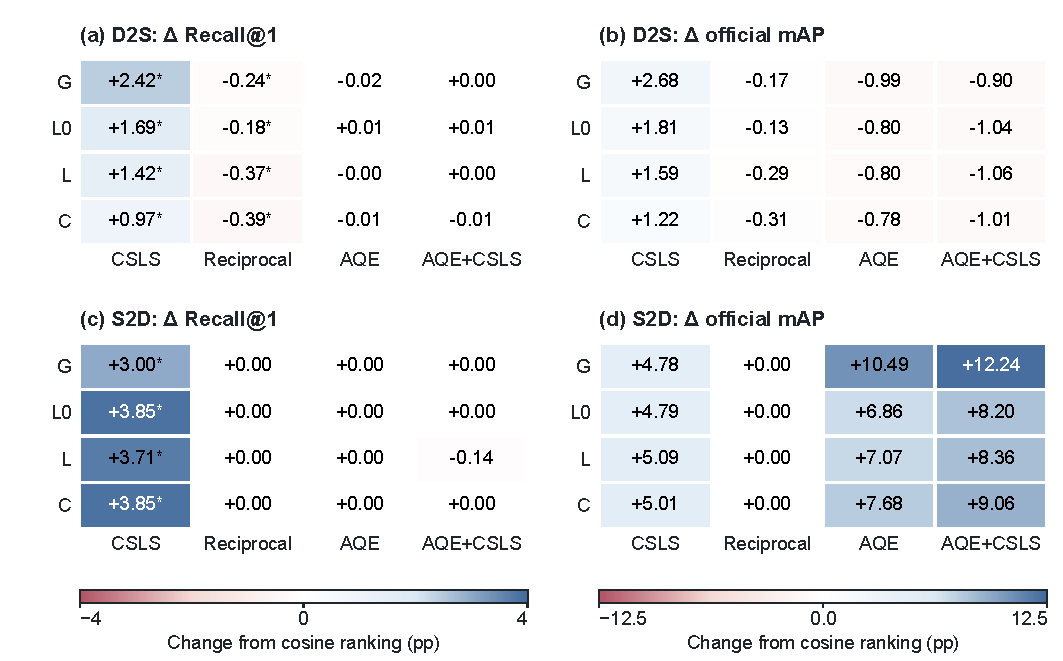
\includegraphics[width=180mm]{figures/journal_20260914/fig06_rule_sensitivity.pdf}
  \caption{Controlled retrieval-rule sensitivity using the same frozen public-baseline features. The upper and lower rows show D2S and S2D, respectively. Cells show changes from cosine ranking in (a,c) Recall@1 and (b,d) official trapezoidal mAP, in percentage points. All rules use $k=10$. Within each metric, both directions share the same zero-centered color scale; the two metrics have different ranges. Blue denotes improvement and red denotes degradation. Asterisks indicate Recall@1 comparisons that pass Holm correction at 0.05 across 32 paired tests; mAP changes are descriptive. Method abbreviations follow Fig.~\ref{fig:exact-public-effects}.}
  \label{fig:retrieval-rule-sensitivity}
\end{figure*}

\subsection{Retrieval-Rule Sensitivity}

Using the same four frozen public feature sources, we separately compared
cosine ranking; cross-domain similarity local scaling (CSLS), adapted from
local neighborhood scaling
\cite{csls2018}; a reciprocal-neighbor bonus, treated as a distinct controlled
variant rather than full k-reciprocal encoding \cite{rerank2017}; a
rank-weighted average query-expansion heuristic, conceptually related to
classical visual automatic query expansion \cite{aqe2007}; and query expansion
followed by CSLS.  We also evaluated all 15
nonempty equal-weight model subsets after score standardization.  These experiments quantify post-processing and score combination for
the four fixed visual baselines.

Ranking changes affected identification and ranking depth differently.
Figure~\ref{fig:retrieval-rule-sensitivity} separates D2S and S2D in the
upper and lower rows, with Recall@1 and mAP in the left and right columns.  CSLS-k10 increased Recall@1 for every method in both directions by
0.97--3.85 points, and all eight paired changes remained significant after
Holm correction.  Reciprocal-k10 instead reduced D2S Recall@1 by 0.18--0.39
points for all four baselines, with all four reductions remaining
significant.  AQE and AQE+CSLS changed Top-1 correctness by at most 0.14
points, yet increased S2D official mAP by 6.86--12.24 points.  The latter
pattern indicates a redistribution of positive ranks rather than additional
rank-1 identifications; these mAP shifts are descriptive.

The supplementary material retains the complete numerical retrieval-rule,
gallery-scale, and fusion comparison tables.

\begin{figure*}[!t]
  \centering
  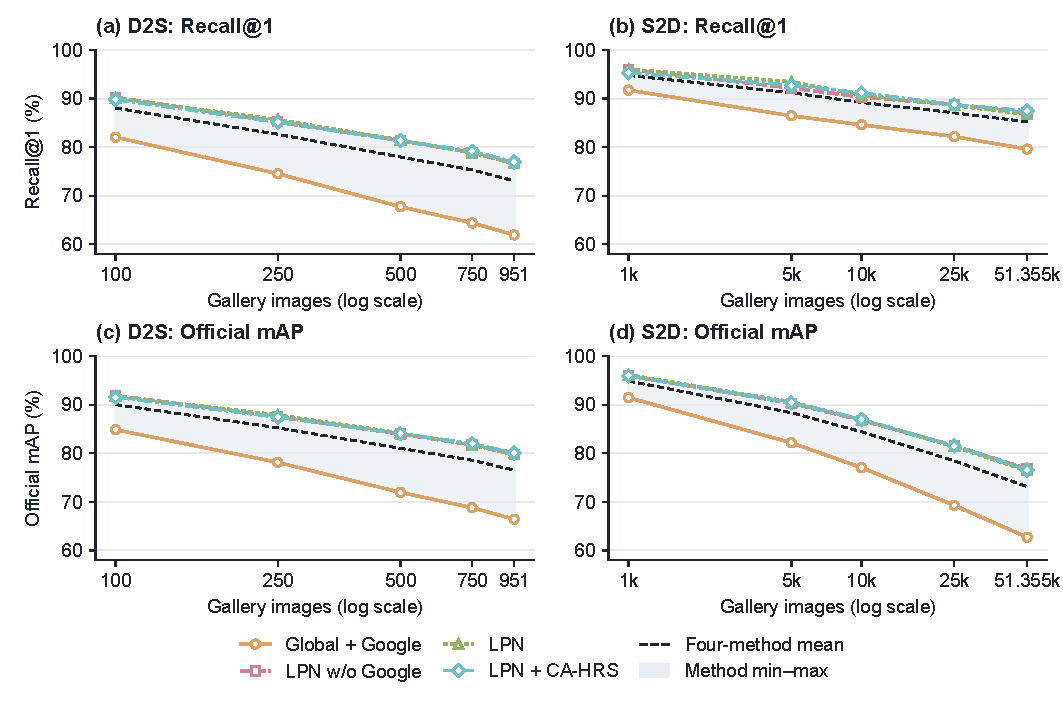
\includegraphics[width=180mm]{figures/journal_20260914/fig07_gallery_scaling.pdf}
  \caption{Gallery-size sensitivity under the controlled vectorized-ranking analysis. (a,b) Recall@1 and (c,d) official trapezoidal mAP for D2S and S2D retrieval, respectively. Colors, marker shapes and line styles identify the four fixed public baselines. Dashed black lines show their arithmetic mean; shading spans the minimum and maximum across methods. Gallery counts use a logarithmic horizontal axis, and all panels share the same performance limits. The near-overlapping LPN trajectories are retained at their original values.}
  \label{fig:gallery-scaling}
\end{figure*}

\subsection{Effect of Gallery Size}
Gallery size produced a large and monotonic difficulty shift.  Averaged over
the four baselines, D2S Recall@1 declined from 88.03\% with 100 candidates to
73.06\% with all 951 candidates, while official mAP declined from 90.01\% to
76.52\%.  S2D Recall@1 declined from 94.76\% with 1,000 candidates to 85.20\%
with all 51,355 candidates; its official mAP fell more sharply, from 94.87\%
to 73.13\%.  The full-gallery method range in the controlled vectorized-ranking analysis
was also substantial: D2S
Recall@1/mAP spanned 61.92--76.94\%/66.43--80.04\%, whereas S2D spanned
79.60--87.45\%/62.73--76.79\%.  The 0.01-point differences from the exact per-query reproduction table arise
from the distinct near-tie ranking implementations. The envelopes span the minimum and maximum of the four method values. Figure~\ref{fig:gallery-scaling} separates the two directions and metrics and retains each method's complete trajectory. It
therefore shows that full-gallery ranking depth, particularly in S2D, is
substantially harder than reduced-gallery identification.

\begin{figure*}[!t]
  \centering
  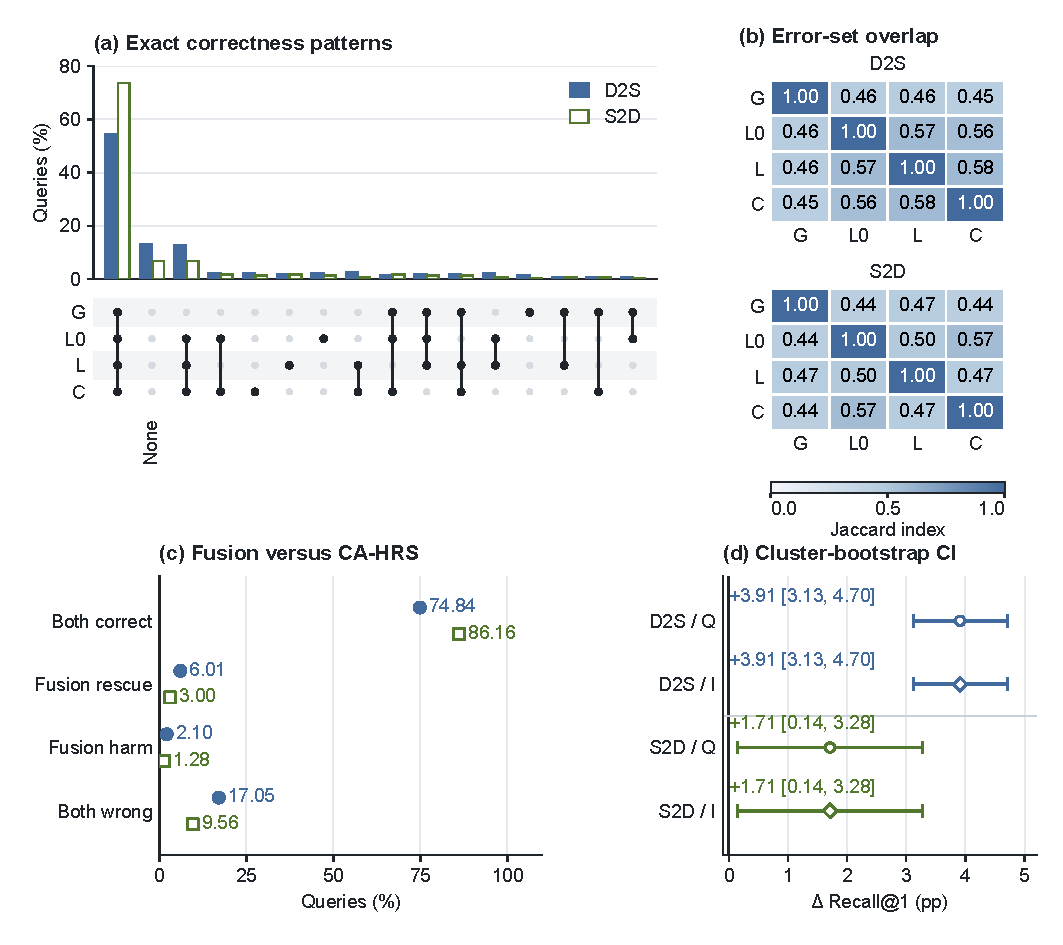
\includegraphics[width=180mm]{figures/journal_20260914/fig08_complementarity.pdf}
  \caption{Query-level complementarity and post-hoc fusion behavior on path-aligned University-1652 queries. (a) All 16 exact Top-1 correctness patterns. Each column of the UpSet matrix specifies which baselines are correct: dark dots indicate inclusion, pale dots indicate absence, and the empty column denotes no correct baseline. Paired bars show the fraction of queries for each direction. (b) Error-set Jaccard overlap, with a common 0--1 scale. (c) The complete partition into both correct, fusion rescue, fusion harm and both wrong relative to CA-HRS. (d) Fusion-minus-CA-HRS Recall@1 differences with 95\% identity-cluster bootstrap intervals from 10,000 resamples, under query-weighted (Q) and identity-balanced (I) estimands. The subset was selected on the same evaluation set; intervals are conditional and do not correct selection optimism. Method abbreviations follow Fig.~\ref{fig:exact-public-effects}.}
  \label{fig:public-baseline-complementarity}
\end{figure*}

\subsection{Error Complementarity and Fusion Cost}

The four cosine baselines made non-identical Top-1 errors on the path-aligned
University-1652 queries. Figure~\ref{fig:public-baseline-complementarity}(a)
shows all 16 exact correctness patterns as an UpSet display, and panel (b)
quantifies overlap between the error sets.  The
retained three-model fusion reached 80.85\% D2S and 89.16\% S2D Recall@1,
rescuing 2,275 and 21 CA-HRS failures while harming 795 and 9 previously
correct queries.  Identity-cluster bootstrap sensitivity analysis (10,000
replicates) gave fusion-minus-CA-HRS differences of 3.91 percentage points
(95\% CI, 3.13--4.70) for D2S and 1.71 points (95\% CI, 0.14--3.28) for S2D.
The subset was selected on these evaluation queries, so the intervals
condition on that selection and quantify sampling variability within the
retained subset.

\begin{figure*}[!t]
  \centering
  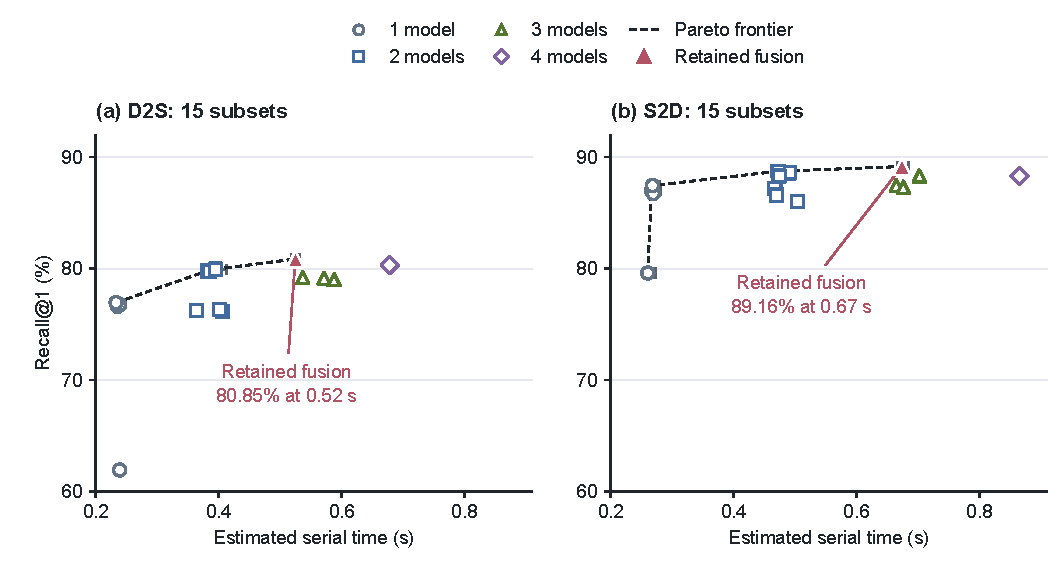
\includegraphics[width=180mm]{figures/journal_20260914/fig09_accuracy_cost.pdf}
  \caption{Accuracy--cost trade-off across all 15 nonempty equal-weight score-fusion subsets of the four public baselines, separately for (a) D2S and (b) S2D. Marker shape and color encode model count. The dashed line joins the Pareto-optimal subsets, and the filled triangle identifies the retained three-model fusion: LPN without Google, LPN and LPN + CA-HRS. Horizontal intervals reproduce the selected overhead Q1--Q3 ranges from 20 timing repetitions with recorded median cosine-ranking time held fixed. They summarize the serial timing proxy obtained from ranking time and fusion overhead. The subset was selected post hoc on the evaluation set.}
  \label{fig:fusion-tradeoff}
\end{figure*}

Figure~\ref{fig:fusion-tradeoff} summarizes the accuracy--cost relation.
Table~\ref{tab:formal-best-fusion} gives the corresponding paired comparisons.
The selected three-model fusion had higher Top-1 recall and average
precision than LPN+CA-HRS on the same evaluation queries.  D2S Recall@1/mAP changed from
76.94/80.04\% to 80.85/83.52\%, whereas S2D changed from 87.45/76.58\% to
89.16/80.46\%. These gains required three 2,048-dimensional descriptors, with
estimated serial retrieval times of 0.52 s (D2S) and 0.67 s (S2D).
The estimates add recorded median cosine-ranking time to repeatedly measured
fusion overhead. The corresponding intervals, 0.519--0.532 s and
0.666--0.684 s, reflect overhead variability with cosine time held fixed;
they summarize the variability of the measured fusion overhead.

\begin{table*}[!p]
\centering
\small
\caption{Post-hoc three-model score fusion versus LPN+CA-HRS on
path-aligned University-1652 queries. Confidence intervals use paired query
resampling; the text separately reports identity-cluster sensitivity.
Intervals and tests are conditional on the selected fusion subset.}
\label{tab:formal-best-fusion}
\begin{tabular}{lrrrrrrr}
\toprule
Direction & Single R@1 & Fusion R@1 & $\Delta$R@1 [95\% CI]
& Single mAP & Fusion mAP & $\Delta$mAP & $p_{\rm Holm}$ \\
\midrule
D2S & 76.94 & 80.85 & +3.91 [3.62, 4.19]
    & 80.04 & 83.52 & +3.48 & $2.71{\times}10^{-163}$ \\
S2D & 87.45 & 89.16 & +1.71 [0.14, 3.28]
    & 76.58 & 80.46 & +3.88 & 0.0428 \\
\bottomrule
\end{tabular}
\end{table*}


\begin{figure*}[!t]
  \centering
  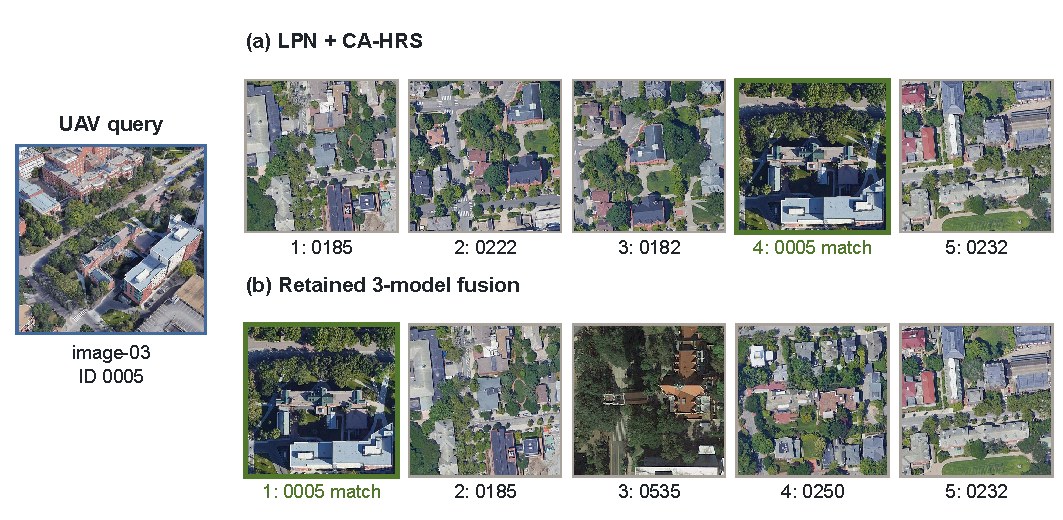
\includegraphics[width=180mm]{figures/journal_20260914/fig10_qualitative.pdf}
  \caption{A deterministic D2S retrieval example from the public-baseline features. The UAV image is the lexicographically first path-aligned query for which CA-HRS fails at Top-1 and the retained score fusion succeeds. Panels compare (a) LPN + CA-HRS and (b) the retained three-model fusion. Labels give rank and gallery identity; green borders and the word ``match'' identify the correct location. Fusion moves identity 0005 from rank 4 to rank 1. All source images are shown in full, with no cropping, enhancement or image-content modification.}
  \label{fig:qualitative-fusion-rescue}
\end{figure*}

\subsection{Qualitative Retrieval Behavior}
Figure~\ref{fig:qualitative-fusion-rescue} shows a Query+Top-5 diagnostic constructed from the frozen
public-baseline features.  The displayed case is the lexicographically first path-aligned D2S query
for which CA-HRS is wrong at Top-1 and the retained fusion is correct; this
selection rule is applied before image display.  CA-HRS ranks the correct identity
0005 fourth, behind three visually similar locations; fusion moves identity
0005 to rank 1.  The remaining Top-5 candidates contain repeated structures that resemble
the query, illustrating the ambiguity among the retrieved gallery images.

\section{Discussion}

\subsection{Semantic Inputs and Descriptor Learning}

The fixed vocabulary supplies a repeatable input interface, and separate
branches preserve the content/style grouping through descriptor construction.
The completed comparisons show that this design does not yield a general
accuracy advantage under the frozen protocol: Full is lower than Visual in
10 of 11 official tasks for mean R@1 and mAP, and in every transfer task for
mean R@1. Street2S provides a small official exception at low absolute
accuracy. These are observations about the evaluated configurations; they
do not isolate a causal failure mechanism or establish a compensating
efficiency, robustness or calibration advantage.

The corruption and query diagnostics need their own interpretation.
Retention is normalized by each model's clean performance, shared Visual
margin masks condition the T4 comparison, and T5 variants can select
different query members. A favorable conditional value cannot replace the
full-task comparison. Independent per-image encoding still permits gallery
descriptors to be computed in advance, but a deployment benefit requires
corresponding measurements.

This design also defines concrete modeling trade-offs. Fixed vocabularies
provide compact, repeatable inputs but omit detailed object geometry and
continuous spatial relations. Their scores depend on the prompt set and the
frozen CLIP embedding space; content and style probabilities can remain
correlated. Learned probability encoders and descriptor fusion introduce
additional parameters. A visual model with comparable capacity is therefore
a useful complement to the branch comparisons when attributing an observed
effect to semantic information.

\subsection{Ranking, Gallery Composition, and Model Combination}

The visual-baseline experiments show that the retrieval procedure affects
different parts of the ranking. CSLS changes the leading match across both
directions, whereas query expansion mainly improves the placement of
additional positives in S2D. Increasing the gallery introduces more
competing images and lowers both recall and average precision. These
observations support reporting the full gallery, ranking rule, and both
metrics alongside the descriptor architecture.

The three-model visual fusion combines partially overlapping error sets.
Its rescue and harm counts explain the net improvement over CA-HRS on the
analyzed queries. Because the subset was selected from the same evaluation
set, these results describe retrospective complementarity. A deployed
ensemble requires a subset fixed on separate validation data. The measured
overhead and serial timing estimate also distinguish the cost of combining
stored scores from the cost of encoding images with multiple networks.

Location identity is another relevant unit of analysis. University-1652
D2S and Street2S and the SUES-200 UAV-to-satellite tasks contain repeated
queries per location. Query-level intervals treat these images as
independent observations; identity-cluster resampling retains their shared
location membership. The reported fusion analysis includes this cluster
analysis, while the broader public-baseline comparisons use query-paired
inference. Both the sampling unit and the measured retrieval direction
belong in the interpretation of an effect.

\subsection{Extension to Operational Localization}

The benchmarks evaluate image identity retrieval across campus and urban
scenes. Continuous-region and non-centered localization, as studied in
Game4Loc \cite{game4loc2025}, introduces additional spatial uncertainty.
Metric pose estimation requires geometric verification after retrieval.
Here, the controlled-corruption comparison also changes Full's evidence
path, so it does not isolate only a pixel transformation. Adverse-weather
flights further combine weather, motion,
visibility, and capture decisions. Extending the framework to these
settings requires data and measurements at the corresponding spatial and
environmental scales.

\section{Conclusion}

We evaluated fixed content and acquisition-style probability inputs within
a shared UAV--satellite retrieval framework. The completed official and
transfer matrices retain the full task set and three training seeds. Full
has lower mean R@1 and mAP than Visual on 10 of 11 official tasks and lower
mean R@1 on all 11 transfer tasks; the low-accuracy Street2S exception does
not support a general fusion advantage. Seed-1 corruption and clean-query
diagnostics describe relative retention and conditional retrieval under
different evidence and query-membership definitions. Together, the results
provide a measured assessment of this fixed semantic interface, while the
separate public-baseline analysis retains its own ranking and post-hoc
fusion conclusions.

\FloatBarrier
\clearpage
% Start the bibliography on a normal page after flushing the remaining floats.
\bibliographystyle{IEEEtran_lgm_display}
\bibliography{ieee_controls,refs}

\end{document}
